\documentclass[12pt]{report}

\usepackage[top=1in, bottom=1.25in, left=1.25in, right=1.25in]{geometry}

\usepackage{siunitx}
\usepackage{hyperref}
\usepackage[all]{hypcap}        % needed to help hyperlinks direct correctly;
\usepackage{xfrac}
\usepackage{adjustbox}
\usepackage{pdfpages}

% Drawings
\usepackage{tikz}
\usetikzlibrary{shapes,arrows}

% Source Code
\usepackage{listings}
\usepackage{color}

% Chapter Title, fix to amke it look better
\usepackage{titlesec}
\titleformat
{\chapter} % command
[display] % shape
{\bfseries\Large\itshape} % format
{\centering Chapter \thechapter} % label
{0.5ex} % sep
{
    \rule{\textwidth}{1pt}
    \vspace{1ex}
    \centering
} % before-code
[
\vspace{-0.5ex}%
\rule{\textwidth}{0.3pt}
] % after-code

\definecolor{mygreen}{rgb}{0,0.6,0}
\definecolor{mygray}{rgb}{0.5,0.5,0.5}
\definecolor{mymauve}{rgb}{0.58,0,0.82}

\lstset{ %
  backgroundcolor=\color{white},   % choose the background color; you must add \usepackage{color} or \usepackage{xcolor}; should come as last argument
  basicstyle=\footnotesize,        % the size of the fonts that are used for the code
  breakatwhitespace=false,         % sets if automatic breaks should only happen at whitespace
  breaklines=true,                 % sets automatic line breaking
  captionpos=b,                    % sets the caption-position to bottom
  commentstyle=\color{mygreen},    % comment style
  deletekeywords={...},            % if you want to delete keywords from the given language
  escapeinside={\%*}{*)},          % if you want to add LaTeX within your code
  extendedchars=true,              % lets you use non-ASCII characters; for 8-bits encodings only, does not work with UTF-8
  frame=single,	                   % adds a frame around the code
  keepspaces=true,                 % keeps spaces in text, useful for keeping indentation of code (possibly needs columns=flexible)
  keywordstyle=\color{blue},       % keyword style
  language=Octave,                 % the language of the code
  morekeywords={*,...},           % if you want to add more keywords to the set
  numbers=left,                    % where to put the line-numbers; possible values are (none, left, right)
  numbersep=5pt,                   % how far the line-numbers are from the code
  numberstyle=\tiny\color{mygray}, % the style that is used for the line-numbers
  rulecolor=\color{black},         % if not set, the frame-color may be changed on line-breaks within not-black text (e.g. comments (green here))
  showspaces=false,                % show spaces everywhere adding particular underscores; it overrides 'showstringspaces'
  showstringspaces=false,          % underline spaces within strings only
  showtabs=false,                  % show tabs within strings adding particular underscores
  stepnumber=2,                    % the step between two line-numbers. If it's 1, each line will be numbered
  stringstyle=\color{mymauve},     % string literal style
  tabsize=2,	                   % sets default tabsize to 2 spaces
  title=\lstname                   % show the filename of files included with \lstinputlisting; also try caption instead of title
}

% Images in figures
\usepackage{graphicx}
\newcommand{\fig}[3]{
  \begin{figure}[!h]
      \centering
      \includegraphics[width=0.8\textwidth]{#1}
      \caption{#2}
      \label{fig:#3}
  \end{figure}
}

% Landscape
\usepackage{pdflscape}

% Bill of Materials product
% \product{item,href,QTY,unitPrice,extendedPrice}
\newcommand{\product}[6]{
    {#1} & {#2} & {#3} & {#4} & {#5} & {#6} \\
}

\title{Muon Telescope}
\author{Sawaiz Syed}

\begin{document}

\maketitle 
\tableofcontents{}

\begin{abstract}
    The assembly, software, and operation of a three paddle plastic scintillator detector. 
\end{abstract}

\pagebreak
\chapter{Components}
\section{Scintillator Panel}
Large scintillator panel with embedded fibre loop to channel light to attached photo-sensor. The tile has a loop pattern with a single fibre to attempt to gather light from as much of the effective area of scintillator and minimize losses from tight curves and open fibre ends. The fibre groove follows along the top surface and comes out perpendicular to end face. A rendering of a assembled panel is shown in Figure~\ref{fig:assembledPanel}.

\fig{./tex/scintillatorPanel/img/scintillatorPanel}{Fully assembled Scintillator panel.}{assembledPanel}

\subsection{Theory}
The scintillator panel is a doped plastic (available from many suppliers \href{http://www.eljentechnology.com/}{Eljen} being the one used in our assemblies) that emits light in response to being struck by an electron, alpha particle, ion, or high energy photon. The light emitted (blue in our case) is then expected to hit the embedded fibre that can absorb that light, and retransmit at the lower green frequency based on the characteristics of the fibre. This green light is captured and guided by the fibre to the end of finger where it can be read out. Each event is expected to produce about 30 photons, with a lower number reaching the sensor placed on the fibre side. The outer surface has coatings applied to shield from external light and attempt to maximise efficiency by reflecting internal light. A exploded view of all the components is shown in Figure~\ref{fig:explodedPanel}.

\subsection{Assembly}
Currently the parts must be hand assembled although further production may yield an injection moulding scheme. The following lists the procedure to construct a single plate.

\subsubsection{Milling}
The fingers are cut from 10mm thick scintillator and are $\SI{145}{\milli\meter}$ x $\SI{145}{\milli\meter}$. The groove is cut with a ball mill under water flow to prevent deformation of the plastic due to heat. The milled sides are then polished (Novus plastic polish works well) and then are washed with alcohol.

\subsubsection{Gluing}
The optical fibres are cut to length (score and breaking) and the end is polished. It is placed into the groove with a two-part optical cement. This binds the fibre to the milled plastic providing an optical bond. Forcing the fibre to match the contour milled.

\fig{./tex/scintillatorPanel/img/scintillatorPaneExploded}{Exploded view showing coatings and fibre.}{explodedPanel}

\subsubsection{Covering}
The fingers are then covered with either degreased aluminium foil and electrical tape or a coating of reflective spray followed by a dip inside rubberized coating (successful tests have been done with \href{http://www.hobbyrecreationproducts.com/collections/spazstix-ultimate-mirror-chrome}{Spaz Stix Ultimate Mirror Chrome} and \href{https://plastidip.com/}{Plasti Dip}) providing a more even surface finish and reduced labour. This covering shields external light, and provides higher efficiency by capturing stray photons by reflecting them back towards the fibre optic. 

\pagebreak

\section{MPPC Sensor}

The board stack has a MPPC, preamp, temperature sensor, and LED. Having the pre-amp on board, just millimetres from the sensor allows excellent signal integrity, even in high noise environments. Also, having the temperature sensor on the sensor, allows for fine adjustment due to local temperature fluctuations, as the gain is dependent on temperature and bias voltage, a constant gain can be maintained by changing the bias in response to temperature.

\fig{./tex/mppcSensor/img/mppcSensorISOAssembled}{Assembled MPPC sensor board stack.}{assembledStack}

\subsection{Hardware}
This board houses a surface mount $\SI{2.0}{\milli\meter}$ MPPC by Hamamatsu. Specifically, \texttt{S13360-20**VE} series. The signal is amplified with a TI OPA846 op-amp. There is a LED as well as a 100K NTC thermistor. The boards are all $\SI{7}{\milli\meter}$ tall, $\SI{25}{\milli\meter}$ wide and approximately $\SI{6.4}{\milli\meter}$ in depth without the pins. The spacer board blocks out excess light from reaching the MPPC, and provides isolation from the LED forcing it to go through the scintillator. It is attached with two 4-40 screws that can go directly into scintillator or a mounting block.

\begin{table}[h]
    \centering
    \begin{adjustbox}{width=\textwidth,center}
        \begin{tabular}{lllllrrr}
            \multicolumn{8}{ c }{MPPC High Voltage BOM} \\ \hline
            \textbf{Ref-Des} & \textbf{Function}    & \textbf{Description}               & \textbf{P/N}                 & \textbf{Digikey P/N}   & \textbf{QTY} & \textbf{Unit Price} & \textbf{Ext Price}\\ \hline \hline
            C9, C10        & Op-amp Power Filter    & CAP CER 1UF 25V X5R 0402           & \texttt{GRM155R61E105MA12D}  & \href{http://search.digikey.com/scripts/DkSearch/dksus.dll?Detail&name=490-10018-1-ND}{\texttt{490-10018-1-ND}}  & 1     & 0.03250    & 0.03   \\
            C11            & HV Filter              & CAP CER 0.047UF 50V X7R 0402       & \texttt{GRM155R71H473KE14D}  & \href{http://search.digikey.com/scripts/DkSearch/dksus.dll?Detail&name=490-10702-1-ND}{\texttt{490-10702-1-ND}}  & 1     & 0.01320    & 0.01   \\
            C7             & Decoupling             & CAP CER 1UF 10V X5R 0603           & \texttt{CL10A105KP8NNNC   }  & \href{http://search.digikey.com/scripts/DkSearch/dksus.dll?Detail&name=1276-1182-1-ND}{\texttt{1276-1182-1-ND}}  & 1     & 0.01400    & 0.01   \\
            C8             & Decoupling             & CAP CER 10UF 10V X5R 0603          & \texttt{GRM188R61A106ME69D}  & \href{http://search.digikey.com/scripts/DkSearch/dksus.dll?Detail&name=490-10475-1-ND}{\texttt{490-10475-1-ND}}  & 1     & 0.06560    & 0.07   \\
            D1             & MPPC                   & 2.0mmx2.0mm MPPC                   & \texttt{S13360-2050VE     }  & \href{http://www.hamamatsu.com/us/en/community/mppc/4400/S13360-2050VE/index.html    }{\texttt{S13360-2050VE }}  & 1     & 22.00000   & 22.00  \\
            D2             & Led                    & LED GREEN CLEAR 0603 R/A SMD       & \texttt{LTST-S270GKT      }  & \href{http://search.digikey.com/scripts/DkSearch/dksus.dll?Detail&name=160-1475-1-ND }{\texttt{160-1475-1-ND }}  & 1     & 0.11220    & 0.11   \\
            J1,J2          & Spring Connector       & BATTERY CONN 1.2H 1.6MM DR 4CKT    & \texttt{788640001         }  & \href{http://search.digikey.com/scripts/DkSearch/dksus.dll?Detail&name=WM11203CT-ND  }{\texttt{WM11203CT-ND  }}  & 2     & 0.25470    & 0.51   \\
            R9, R10        & Op-amp Power Filter    & RES SMD 10 OHM 5\% 1/16W 0402      & \texttt{RC0402JR-0710RL   }  & \href{http://search.digikey.com/scripts/DkSearch/dksus.dll?Detail&name=311-10JRCT-ND }{\texttt{311-10JRCT-ND }}  & 2     & 0.00470    & 0.01   \\
            R2             & NTC Therm              & THERMISTOR NTC 100KOHM 0.5\% 0603  & \texttt{NCP18WF104D03RB   }  & \href{http://search.digikey.com/scripts/DkSearch/dksus.dll?Detail&name=490-11811-1-ND}{\texttt{490-11811-1-ND}}  & 1     & 0.31270    & 0.31   \\
            R11, R12, R14  & 51 ohm Term            & RES SMD 51 OHM 5\% 1/16W 0402      & \texttt{RC0402JR-0751RL   }  & \href{http://search.digikey.com/scripts/DkSearch/dksus.dll?Detail&name=311-51JRCT-ND }{\texttt{311-51JRCT-ND }}  & 3     & 0.00470    & 0.01   \\
            R13, R15       & Op-amp Gain/ HV Filter & RES SMD 1K OHM 0.1\% 1/16W 0402    & \texttt{RT0402BRD071KL    }  & \href{http://search.digikey.com/scripts/DkSearch/dksus.dll?Detail&name=YAG1386CT-ND  }{\texttt{YAG1386CT-ND  }}  & 2     & 0.12760    & 0.26   \\
            U1             & Op-Amp                 & IC OPAMP VFB 1.75GHZ SOT23-5       & \texttt{OPA846IDBVT       }  & \href{http://search.digikey.com/scripts/DkSearch/dksus.dll?Detail&name=296-14776-1-ND}{\texttt{296-14776-1-ND}}  & 1     & 3.74460    & 3.74   \\
            J3             & Output Header          & MINITEK                            & \texttt{98424-F52-08ALF   }  & \href{http://search.digikey.com/scripts/DkSearch/dksus.dll?Detail&name=609-5175-1-ND }{\texttt{609-5175-1-ND }}  & 1     & 1.04000    & 1.04   \\ \hline
            \multicolumn{5}{ r }{ \href{http://www.oshpark.com/}{PCB Manufacture}}                                                                                                                                                         & 3     & 1.35000    & 4.05   \\ 
            \multicolumn{5}{ r }{ \href{http://www.smallbatchassembly.com/}{Assembly}}                                                                                                                                                     & 1     & 5.38000    & 5.38   \\ \cline{5-8}
            \multicolumn{5}{ r }{ Testing (Labour)}                                                                                                                                                                                        & 0.05  & 30.00000   & 1.50   \\ 
            \multicolumn{7}{ r }{ Subtotal}                                                                                                                                                                                                                     & 39.05  \\
        \end{tabular}
    \end{adjustbox}
    \caption{Bill of Materials, all prices in USD.}
    \label{tab:mppcSesnorBOM}
\end{table}

\fig{./tex/mppcSensor/img/mppcSensorISO2}{Exploded view of MPPC sensor side.}{iso2}
\fig{./tex/mppcSensor/img/sensorSchematic}{Schematic of the preamp, D1 is the MPPC.}{sensorSchematic}
\fig{./tex/mppcSensor/img/connectorsSchematic}{The interconnects between the boards as well as the header in the back.}{connectorsSchematic}

\subsection{Cable}
There are eight pins attached to back of the final board. Those pins break out all signals needed. There is a corner mark on the PCB that lies in the top left corner. On single ended signals, \emph{Sig-} is connected to \emph{GND}.

\begin{table}[h]
    \centering
    \begin{adjustbox}{width=\textwidth,center}
        \begin{tabular}{lllllrrr}
            \multicolumn{8}{ c }{Sensor Interface Cable BOM} \\ \hline
            \textbf{Ref-Des} & \textbf{Function}      & \textbf{Description}                    & \textbf{P/N}                 & \textbf{Supplier P/N}   & \textbf{QTY} & \textbf{Unit Price} & \textbf{Ext Price}\\ \hline \hline
            J3-F             & Output Header Jack     &  CONN IDC SOCKET 8POS 2MM GOLD          & \texttt{89361-708LF}         & \href{http://search.digikey.com/scripts/DkSearch/dksus.dll?Detail&name=609-3140-ND}{\texttt{609-3140-ND}}  & 1     & 1.08800    & 1.09   \\
            W1               & 3 foot Ethernet Cable  &  Cat6 28AWG UTP Ethernet Network Cable  & \texttt{14812}               & \href{http://www.monoprice.com/product?p_id=14808}{\texttt{14808}}                                         & 0.5   & 2.29000    & 1.16   \\
            \multicolumn{5}{ r }{ Assembly (Labour)}                                                                                                                                                                                        & 0.1   & 30.00000   & 3.00   \\ 
            \multicolumn{5}{ r }{ Testing (Labour)}                                                                                                                                                                                         & 0.05  & 30.00000   & 1.50   \\ 
            \multicolumn{7}{ r }{ Subtotal}                                                                                                                                                                                                                      & 6.05   \\
        \end{tabular}
    \end{adjustbox}
    \caption{Bill of Materials, all prices in USD.}
    \label{tab:mppcSesnorBOM}
\end{table}

\fig{./tex/mppcSensor/img/mppcSensorPinout}{Pin numbering for Table~\ref{tab:pinOut}.}{mppcSensorPinout}

\begin{table}[h]
    \centering
    \begin{tabular}{ r l l }
        \multicolumn{3}{ c }{Sensor Interface Cable Connections} \\ \hline
        \textbf{Pin} & \textbf{Function} & \textbf{Type} \\ \hline \hline
        1                & Signal -          & Output        \\
        2                & Signal +          & Output        \\
        3                & $+V_{S}$          & Power         \\
        4                & Ground            & Power         \\
        5                & LED               & Input         \\
        6                & $-V_{S}$          & Power         \\
        7                & High Voltage      & Power         \\
        8                & Thermistor        & Output        \\
    \end{tabular}
    \caption{Pinout on the back side with pins facing you and the cut corner on top left.}
    \label{tab:pinOut}
\end{table}

The cable used is a 28AWG CAT6 cable, Monoprice's \href{http://www.monoprice.com/product?p_id=14812}{Slimrun} line is an option. This provides 8 conductors that are twisted pairs, along with an 8P8C connector. Wiring standard used is the following positions.

\begin{table}[h]
    \centering
    \begin{tabular}{ l l l l }
        \textbf{RJ-45 Pin} & \textbf{Cable Colour}  & \textbf{Signal}  & \textbf{Abv}  \\ \hline \hline
        MD0+               & White Orange           & High Voltage     & HV+  \\
        MD0-               & Orange                 & Ground           & GND  \\
        MD1+               & White Green            & Test             & LED  \\
        MD1-               & Blue                   & Thermistor       & TEMP \\
        MD2+               & White Blue             & +Voltage         & +Vcc \\
        MD2-               & Green                  & -Voltage         & -Vcc \\
        MD3+               & White Brown            & Signal+          & Sig+ \\
        MD3-               & Brown                  & Signal-          & Sig- \\
    \end{tabular}
    \caption{Pinout on the back side with pins facing you and the cut corner on top left.}
    \label{tab:cableConnections}
\end{table}

\fig{./tex/mppcSensor/img/mppcSensorISO1}{Exploded view of connector side.}{iso1}

\pagebreak


\section{MPPC High Voltage Supply}

Surface mount module that provides $\SI{52.5}{\volt}$ to $\SI{57.5}{\volt}$ in $\SI{20}{\milli\volt}$ increments. Also contains a 2 input 24bit ADC to allow for closed loop control of the voltage, and read in a thermistor mounted near the sensor. Rendering of a fully assembled module shown in Figure~\ref{fig:withEMIshield}.

\fig{./tex/mppcHighVoltage/img/withEMIshield}{Board rendering with EMI shield.}{withEMIshield}

\subsection{Hardware}
The module uses a MAX1932 APD bias voltage boost converter and NAU7802SGI 24bit Analog to Digital converter (ADC) for reading temperature and output voltage. The complete bill of materials including assembly and testing is detailed in Table~\ref{tab:mppcHighVoltageBOM}.

\begin{table}[h]
    \centering    
    \begin{adjustbox}{width=\textwidth,center}
        \begin{tabular}{lllllrrr}
            \multicolumn{8}{ c }{MPPC High Voltage BOM} \\ \hline
            \textbf{Ref-Des} & \textbf{Function}      & \textbf{Description}                    & \textbf{P/N}                & \textbf{Digikey P/N}   & \textbf{QTY} & \textbf{Unit Price} & \textbf{Ext Price}  \\ \hline \hline
            C1               & Input Decoupling       & 1µF 16V Ceramic Capacitor X7R 1206      & \texttt{160R18W105KV4E    } & \href{http://search.digikey.com/scripts/DkSearch/dksus.dll?Detail&name=709-1068-1-ND    }{\texttt{709-1068-1-ND    }}      & 1     & 0.0890     & 0.09  \\
            C2               & Boost Capacitor        & 0.047µF 500V Ceramic Capacitor X7R 1206 & \texttt{C1206C473KCRACTU  } & \href{http://search.digikey.com/scripts/DkSearch/dksus.dll?Detail&name=399-6743-1-ND    }{\texttt{399-6743-1-ND    }}      & 1     & 0.1300     & 0.13  \\
            C3               & Pre Filter Capacitor   & 0.10µF 250V Ceramic Capacitor X7R 1206  & \texttt{C1206C104KARACTU  } & \href{http://search.digikey.com/scripts/DkSearch/dksus.dll?Detail&name=399-4674-1-ND    }{\texttt{399-4674-1-ND    }}      & 1     & 0.1485     & 0.15  \\
            C4               & Post Filter Capacitor  & CAP CER 1UF 100V X7R 1206               & \texttt{12061C105KAT2A    } & \href{http://search.digikey.com/scripts/DkSearch/dksus.dll?Detail&name=478-6226-1-ND    }{\texttt{478-6226-1-ND    }}      & 1     & 0.1570     & 0.16  \\
            C5               & Compensation Capacitor & CAP CER 0.22UF 16V Y5V 0402             & \texttt{CL05F224ZO5NNNC   } & \href{http://search.digikey.com/scripts/DkSearch/dksus.dll?Detail&name=1276-1060-1-ND   }{\texttt{1276-1060-1-ND   }}      & 1     & 0.0112     & 0.01  \\
            D1               & Boost Diode            & DIODE GEN PURP 100V 200MA SOD80         & \texttt{LL4148            } & \href{http://search.digikey.com/scripts/DkSearch/dksus.dll?Detail&name=LL4148FSCT-ND    }{\texttt{LL4148FSCT-ND    }}      & 1     & 0.0420     & 0.04  \\
            L1               & Boost Inductor         & FIXED IND 150UH 320MA 2.4 OHM           & \texttt{SRN4018-151M      } & \href{http://search.digikey.com/scripts/DkSearch/dksus.dll?Detail&name=SRN4018-151MCT-ND}{\texttt{SRN4018-151MCT-ND}}      & 1     & 0.2400     & 0.24  \\
            L2               & Smoothing Inductor     & FIXED IND 330UH 90MA 15.99 OHM          & \texttt{CBC2518T331K      } & \href{http://search.digikey.com/scripts/DkSearch/dksus.dll?Detail&name=587-3059-1-ND    }{\texttt{587-3059-1-ND    }}      & 1     & 0.1400     & 0.14  \\
            Q1               & Boost Switch           & MOSFET N-CH 100V 0.17A SOT-23           & \texttt{BSS123L           } & \href{http://search.digikey.com/scripts/DkSearch/dksus.dll?Detail&name=BSS123LCT-ND     }{\texttt{BSS123LCT-ND     }}      & 1     & 0.1032     & 0.10  \\
            R1               & Current Sens Resistor  & RES SMD 806 OHM 0.1\% 1/16W 0402        & \texttt{RT0402BRD07806RL  } & \href{http://search.digikey.com/scripts/DkSearch/dksus.dll?Detail&name=YAG1481CT-ND     }{\texttt{YAG1481CT-ND     }}      & 1     & 0.1276     & 0.13  \\
            R2, R6           & Adjustment Span/Temp   & RES SMD 100K OHM 0.1\% 1/16W 0402       & \texttt{RT0402BRD07100KL  } & \href{http://search.digikey.com/scripts/DkSearch/dksus.dll?Detail&name=YAG1343CT-ND     }{\texttt{YAG1343CT-ND     }}      & 2     & 0.1276     & 0.26  \\
            R3               & Minimum Voltage Res    & RES SMD 2.37KOHM 0.1\% 1/16W 0402       & \texttt{CPF0402B2K37E1    } & \href{http://search.digikey.com/scripts/DkSearch/dksus.dll?Detail&name=A102770CT-ND     }{\texttt{A102770CT-ND     }}      & 1     & 0.2082     & 0.21  \\
            R4               & DAC Resistor           & RES SMD 24.9KOHM 0.1\% 1/16W 0402       & \texttt{RT0402BRD0724K9L  } & \href{http://search.digikey.com/scripts/DkSearch/dksus.dll?Detail&name=YAG1393CT-ND     }{\texttt{YAG1393CT-ND     }}      & 1     & 0.1276     & 0.13  \\
            R5               & Compensation Res       & RES SMD 20 OHM 0.1\% 1/16W 0402         & \texttt{CPF0402B20RE1     } & \href{http://search.digikey.com/scripts/DkSearch/dksus.dll?Detail&name=A102706CT-ND     }{\texttt{A102706CT-ND     }}      & 1     & 0.1973     & 0.20  \\
            U1               & Boost Controller       & IC SUPPLY BIAS APD 12-TQFN              & \texttt{MAX1932ETC+T      } & \href{http://search.digikey.com/scripts/DkSearch/dksus.dll?Detail&name=MAX1932ETC+TCT-ND}{\texttt{MAX1932ETC+TCT-ND}}      & 1     & 7.2828     & 7.28  \\
            U2               & ADC                    & IC ADC 24BIT I2C/SRL 16-SOP             & \texttt{NAU7802SGI        } & \href{http://search.digikey.com/scripts/DkSearch/dksus.dll?Detail&name=NAU7802SGI-ND    }{\texttt{NAU7802SGI-ND    }}      & 1     & 1.3442     & 1.34  \\
            C6               & 0.1uF                  & 0.10µF 10V Ceramic Capacitor X5R 0402   & \texttt{CL05A104KP5NNNC   } & \href{http://search.digikey.com/scripts/DkSearch/dksus.dll?Detail&name=1276-1022-1-ND   }{\texttt{1276-1022-1-ND   }}      & 2     & 0.0048     & 0.01  \\
            C7               & 1uF                    & 1µF 6.3V Ceramic Capacitor X6S 0402     & \texttt{GRM155C80J105KE15D} & \href{http://search.digikey.com/scripts/DkSearch/dksus.dll?Detail&name=490-6281-1-ND    }{\texttt{490-6281-1-ND    }}      & 1     & 0.0055     & 0.01  \\
            C8               & 10uF                   & 10µF 6.3V Ceramic Capacitor X5R 0603    & \texttt{GRM155R60G106ME44D} & \href{http://search.digikey.com/scripts/DkSearch/dksus.dll?Detail&name=490-10693-1-ND   }{\texttt{490-10693-1-ND   }}      & 1     & 0.0380     & 0.04  \\
            S1               & RF Shield              & RFI SHIELD CAN 20X15X3MM                & \texttt{S02-20150300      } & \href{http://search.digikey.com/scripts/DkSearch/dksus.dll?Detail&name=952-2632-ND      }{\texttt{952-2632-ND      }}      & 1     & 3.5300     & 3.53  \\
            R7               & 220k 1\%               & RES SMD 220K OHM 1\% 1/16W 0402         & \texttt{RC0402FR-07220KL  } & \href{http://search.digikey.com/scripts/DkSearch/dksus.dll?Detail&name=311-220KLRCT-ND  }{\texttt{311-220KLRCT-ND  }}      & 1     & 0.0054     & 0.01  \\
            R9               & 270k 1\%               & RES SMD 270K OHM 1\% 1/16W 0402         & \texttt{RC0402FR-07270KL  } & \href{http://search.digikey.com/scripts/DkSearch/dksus.dll?Detail&name=311-270KLRCT-ND  }{\texttt{311-270KLRCT-ND  }}      & 1     & 0.0054     & 0.01  \\
            R8               & 10k 0.1\%              & RES SMD 10K OHM 1\% 1/16W 0402          & \texttt{RC0402FR-0710KL   } & \href{http://search.digikey.com/scripts/DkSearch/dksus.dll?Detail&name=311-10.0KLRCT-ND }{\texttt{311-10.0KLRCT-ND }}      & 1     & 0.0054     & 0.01  \\ \hline
            \multicolumn{5}{ r }{ \href{http://www.oshpark.com/}{PCB Manufacture}}                                                                                                                                                                         & 1     & 1.5333     & 1.53  \\ 
            \multicolumn{5}{ r }{ \href{http://www.smallbatchassembly.com/}{Assembly}}                                                                                                                                                                     & 1     & 9.3000     & 9.30  \\ \cline{5-8}
            \multicolumn{5}{ r }{ Testing (Labour)}                                                                                                                                                                                                        & 0.05  & 30.0000    & 1.50  \\ 
            \multicolumn{5}{ r }{ Calibration (Labour)}                                                                                                                                                                                                    & 0.05  & 30.0000    & 1.50  \\ \cline{5-8}
            \multicolumn{7}{ r }{ Subtotal}                                                                                                                                                                                                                                     & 28.03 \\
        \end{tabular}
    \end{adjustbox}
    \caption{Bill of materials All prices in USD.}
    \label{tab:mppcHighVoltageBOM}
\end{table}

\fig{./tex/mppcHighVoltage/img/noShieldFront}{EMI shield removed showing switching region.}{noShieldFront}

\subsubsection{High Voltage}
The module uses a \href{http://datasheets.maximintegrated.com/en/ds/MAX1932.pdf}{MAX1932} APD bias voltage boost converter to create and maintain the output voltage. The voltage range, and step size is dictated with setting \texttt{R2}, \texttt{R3}, and \texttt{R4}. The minimum and maximum voltage set using the equations for on page 7 of the datasheet, and there are 8 bits (256) intermediate values that are possible the corresponding schematic is show in in Figure~\ref{fig:hvSchematic}. The high switching portion was designed with general SMPS design requirements (short high current loops, separated ground planes, EMI shielding) providing a low ripple output ($<\SI{5}{\milli\volt}_{pp}$ ripple) and no significant back EMF.

\fig{./tex/mppcHighVoltage/img/hvSchematic}{Schematic for high voltage boost converter.}{hvSchematic}

\subsubsection{ADC}
The analogue to digital converter is a one designed for high precision and low sampling rate. The \href{http://www.nuvoton.com/resource-files/NAU7802%20Data%20Sheet%20V1.7.pdf}{NAU7802SGI} is marketed at the load sensing market, but the high precision and low sampling rate lends itself well to the closed loop control and monitoring application. The high voltage is divided by 50 and the thermistor is put across a equivalent 100K static resistor to go along with the 100K NTC found on the MPPC sensor module to act as a voltage divider, see Figure~\ref{fig:assemblySchematic} for details.

\fig{./tex/mppcHighVoltage/img/assemblySchematic}{Schematic showing contacts, adc, and high voltage hierarchy block.}{assemblySchematic}

\subsection{Software}
Each module has two buses that run to it, I\textsuperscript{2}C (pronounced I-two-C) and SPI. SPI requires data, clock, and a chip-select meaning each device on the bus will need an independent chip select. I\textsuperscript{2}C devices have a fixed address therefore it is not possible to have multiple devices on the same bus. This can be remedied by placing multiple devices in front of a I\textsuperscript{2}C multiplexer. Table~\ref{tab:pinOut} lists their functions.

\begin{table}[!h]
    \centering
    \begin{tabular}{ r l l }
        \multicolumn{3}{ c }{MPPC High Voltage Pinout} \\
        \hline
        \textbf{Pin} & \textbf{Label} & \textbf{Description}                     \\ \hline \hline
        1            & \texttt{3V3}   & Regulated $\SI{3.3}{\volt}$ in           \\
        2            & \texttt{CS}    & \emph{SPI} bus Chip Select               \\
        3            & \texttt{SCLK}  & \emph{SPI} bus clock                     \\
        4            & \texttt{DIN}   & \emph{SPI} bus data in                   \\
        5            & \texttt{GND}   & Common Ground                            \\
        6            & \texttt{DRDY}  & ADC conversion done                      \\
        7            & \texttt{SCL}   & \emph{I\textsuperscript{2}C} bus clock   \\
        8            & \texttt{SDA}   & \emph{I\textsuperscript{2}C} bus data    \\
    \end{tabular}
    \caption{Pins and thier fuctions.}    
    \label{tab:pinOut}
\end{table}

\subsubsection{High Voltage}
The SPI bus is connected directly to the MAX1932. Chip select is active low and data is sent MSB (most significant bit first). Sending bytes to it sets the voltage. Setting them to \texttt{0x00} turns off the DC-DC converter portion. As values increase to \texttt{0xFF (127)}, the output voltage falls, linearly. Example code for Arduino that cycles through all possible values is shown in Listing~\ref{lst:max1932}.

\lstinputlisting[language=C++, caption="max1932.ino", label={lst:max1932}]{./tex/mppcHighVoltage/source/max1932.ino}

\subsubsection{ADC}
The ADC communicates through the I\textsuperscript{2}C bus, the device address is permanently programmed to \texttt{0101010 (0x2A)}. It is fully compliant with the I\textsuperscript{2}C protocol and the datasheet has the register map (page 28) and protocol description (page 14).

\lstinputlisting[language=C++, caption="nau7802.ino", label={lst:nau7802}]{./tex/mppcHighVoltage/source/nau7802.ino}

\fig{./tex/mppcHighVoltage/img/mppcBack}{Back is flat to allow flush mounting to mother-board.}{mppcBack}

% For appendix Nau7802 Library
\begin{landscape}
\lstinputlisting[language=C++, caption="NAU7802.h", basicstyle=\tiny, , label={lst:nau7802.h}]{./tex/mppcHighVoltage/source/nau7802/nau7802.h}
\lstinputlisting[language=C++, caption="Nau7802.cpp", basicstyle=\tiny, label={lst:nau7802.cpp}]{./tex/mppcHighVoltage/source/nau7802/nau7802.cpp}
\end{landscape}


\section{MPPC Interface}

A single assembled board breaks out singals and provides all the interfaces that 4 MPPC Sesnor boards need. The power to each module is supplied via the MPPC high voltage modules attached board. It is able to be run independently for testing and debugging, or on a backplane with many others for more channels.

\fig{./tex/mppcInterface/img/mppcInterfaceTopISO}{Top view of assembled MPPC interface board.}{mppcInterfaceTopISO}

\subsection{Hardware}
The board attaches directly to a Raspberry Pi using the centered GPIO headers. The Raspberry Pi is mounted to the board via four standoffs. It is a stand alone board requiring no backplane. This board can be mounted via the M5 screw holes around the edge.

\subsubsection{Power}
Power is supplied through two pins on the edge connector, or via the micro USB port on board. There is a 600mA buck regulator that provides power when the USB port is used. The board should be powered by 3.3V and a negative power supply module with convert it to -3.3V for the biasing for the op-amps.

\subsubsection{High Voltage}
High voltage is supplied through a daughter board. Each channel has a independent voltage source that can be temperature modulated and monitored via the on board ADC. Further information about the modules can be found in Section.

\subsubsection{Microcontroller}
The side of the board has a Arduino compatible (\href{http://www.atmel.com/images/Atmel-8271-8-bit-AVR-Microcontroller-ATmega48A-48PA-88A-88PA-168A-168PA-328-328P_datasheet_Complete.pdf}{ATmega328}) microcontroller, along with a USB part, USB to UART converter and other supporting circuitry. The button is connected to the reset pin. The programing port on board is a Tag-Connect 6 pin, and is only used for programing the Arduino bootloader.

\fig{./tex/mppcInterface/img/mppcInterfaceBottom}{Bottom of populated board showing sensors and AVR.}{mppcInterfaceBottom}

\subsubsection{I2C Switch}
As all the ADC modules on the daughter boards have the same address, a 8 channel I2C switch ([TCA9548A](http://www.ti.com/lit/ds/symlink/tca9548a.pdf)) is used to communicate to them independently. The pins attached to it are referenced as master, as the microcontroller is acting as the master controlling it.

\subsubsection{Pinout}
There are eight RJ-45 jacks on the edge of the board, each jack has the following pinout. The signal lines are kept on a single twisted pair so if a differential signal is used, higher signal integrity is maintained. The pinout matches that of the MPPC sensor board.

\fig{./tex/mppcInterface/img/mppcInterfaceBottomISO}{Isometric view of bottom.}{mppcInterfaceBottomISO}

\subsection{Software}
The device acts as both a master and slave device. It takes instructions from an external I2C bus, and executes them on the AVR microcontroller to set voltages, provide telemetry, and preform closed loop control.

\subsubsection{AVR Firmware}
The microcontroller on board takes commands sent to the whole module, and forwards them to each daughterboard. It primary control loop involves reading the temperature, finding the associated required bias voltage based on the temperature and setting the voltage on the high voltage supply, then checking if the output voltage is within specification of the required output, and fixing it if not. This loops for all eight channels. Otherwise there is an instruction queue of commands that come into the module.

\subsubsection{Module}
The master can communicate to up to 128 slave devices the address is set within software. The master can request the temperature, or current voltage of any of the eight channels on board, select between different voltage to temperature curves, and set the bias voltage, or pulse the LED on the modules.

\pagebreak
\section{Frame}

The frame is constructed out of \SI{4}{\meter} of Misumi 2020 aluminium extrution, cast angle brackets, t-nuts, M5 screws, and rubber feet. The assembly process requires only a \SI{4}{\milli\meter} hex key.


\subsection{Construction}
The frame is designed to be easy to assembly, take apart, and modify for diffrent experiments and highly rugged. It is constructed out of metric aluminium extrution and cast aluminium angle brackets, with rubber feet at the bottom. A full bill of materials is shown in Table~\ref{tab:frameBOM}. The panels it is meant to hold fit within the $\SI{20}{\milli\meter}$ extrution hegight, and the remining area is filled ithe a soft tubing spring. The panels are supourted on both sides by $\sfrac{3}{32}$ inch acrylic sheet and a addtion panel provides a mounting location for the electronics. The assembly process requires only a \SI{4}{\milli\meter} hex key, and can be made vibration resistant through the application of threadlocker (blue color code). 

\begin{table}[h]
    \centering
    \begin{adjustbox}{width=\textwidth,center}
        \begin{tabular}{ l  l  l  r  r  r }
            \multicolumn{6}{ c }{Bill of Materials} \\
            \hline
            \textbf{Description} & \textbf{Item} & \textbf{Supplier} & \textbf{QTY} & \textbf{Unit} & \textbf{Ext} \\ \hline \hline
            \product{Aluminium Extrustion}{\href{https://us.misumi-ec.com/vona2/detail/110302683830/?HissuCode=KHFS5-2020-1000&PNSearch=KHFS5-2020-1000&searchFlow=results2products&Keyword=KHFS5-2020-1000}{\texttt{KHFS5-2020-1000}}}{Misumi}{4}{6.41}{25.64}
            \product{Angle Brackets}{\href{https://us.misumi-ec.com/vona2/detail/110300437260/?HissuCode=HBLFSNF5&PNSearch=HBLFSNF5&searchFlow=results2products&Keyword=HBLFSNF5}{\texttt{HBLFSNF5}}}{Misumi}{64}{0.63}{40.32}
            \product{M5 T-Nuts}{\href{https://us.misumi-ec.com/vona2/detail/110302246940/?KWSearch=HNKK5-5&Keyword=HNKK5-5&searchFlow=results2products}{\texttt{HNKK5-5}}}{Misumi}{$\sfrac{156}{100}$}{15.26}{23.81}
            \product{M5x6}{\href{https://www.mcmaster.com/91292a189}{\texttt{91292a189}}}{McMaster-Carr}{$\sfrac{28}{50}$}{4.63}{2.59}
            \product{M5x10}{\href{https://www.mcmaster.com/91292a124}{\texttt{91292A124}}}{McMaster-Carr}{$\sfrac{128}{100}$}{8.15}{11.20}
            \product{M5x25}{\href{https://www.mcmaster.com/91292a129}{\texttt{91292a129}}}{McMaster-Carr}{$\sfrac{4}{25}$}{6.85}{1.10}
            \product{Acrylic Sheet}{\href{https://www.mcmaster.com/8560k182}{\texttt{8560k182}}}{McMaster-Carr}{$\sfrac{7}{6}$}{8.96}{10.45}
            \product{Rubber Feet}{\href{https://www.mcmaster.com/9540K717}{\texttt{9540K717}}}{McMaster-Carr}{$\sfrac{4}{25}$}{7.42}{1.19}
            \hline
            \product{Labor}{}{}{2}{30.00}{60.00}
            \hline
            \multicolumn{5}{r}{\textbf{Subtotal}} & XXX.XX \\
            \multicolumn{5}{r}{\textbf{Tax}} & \%8.000 \\
            \multicolumn{5}{r}{\textbf{Transport}} & \%XX.XX \\
            \multicolumn{5}{r}{\textbf{Total (USD)}} & 189.24 \\
        \end{tabular}
    \end{adjustbox}
    \caption{Materials required for one frame.}
    \label{tab:frameBOM}
\end{table}

\begin{table}[h]
    \centering
    \begin{adjustbox}{width=\textwidth,center}
        \begin{tabular}{ l r r l }
            \multicolumn{4}{ c }{Aluminum Extrustion Cut List} \\
            \hline
            \textbf{Description} & \textbf{QTY} & \textbf{Length (mm)} & \textbf{Note}\\ \hline \hline
            Vertical Beam        & 4            & 396                  & M5 thread tapped one end \SI{20}{\milli\meter} deep\\
            Horizontal Beam      & 16           & 150 \\
        \end{tabular}
    \end{adjustbox}
    \caption{One vertical and four horizontal to be cut from each \SI{1}{\meter} section. \SI{1}{\milli\meter} kerf.}    
    \label{tab:cutList}
\end{table}

\subsubsection{Assembly}
Insert assembly PDF output form Illistrator

\pagebreak
\chapter{Assembly}
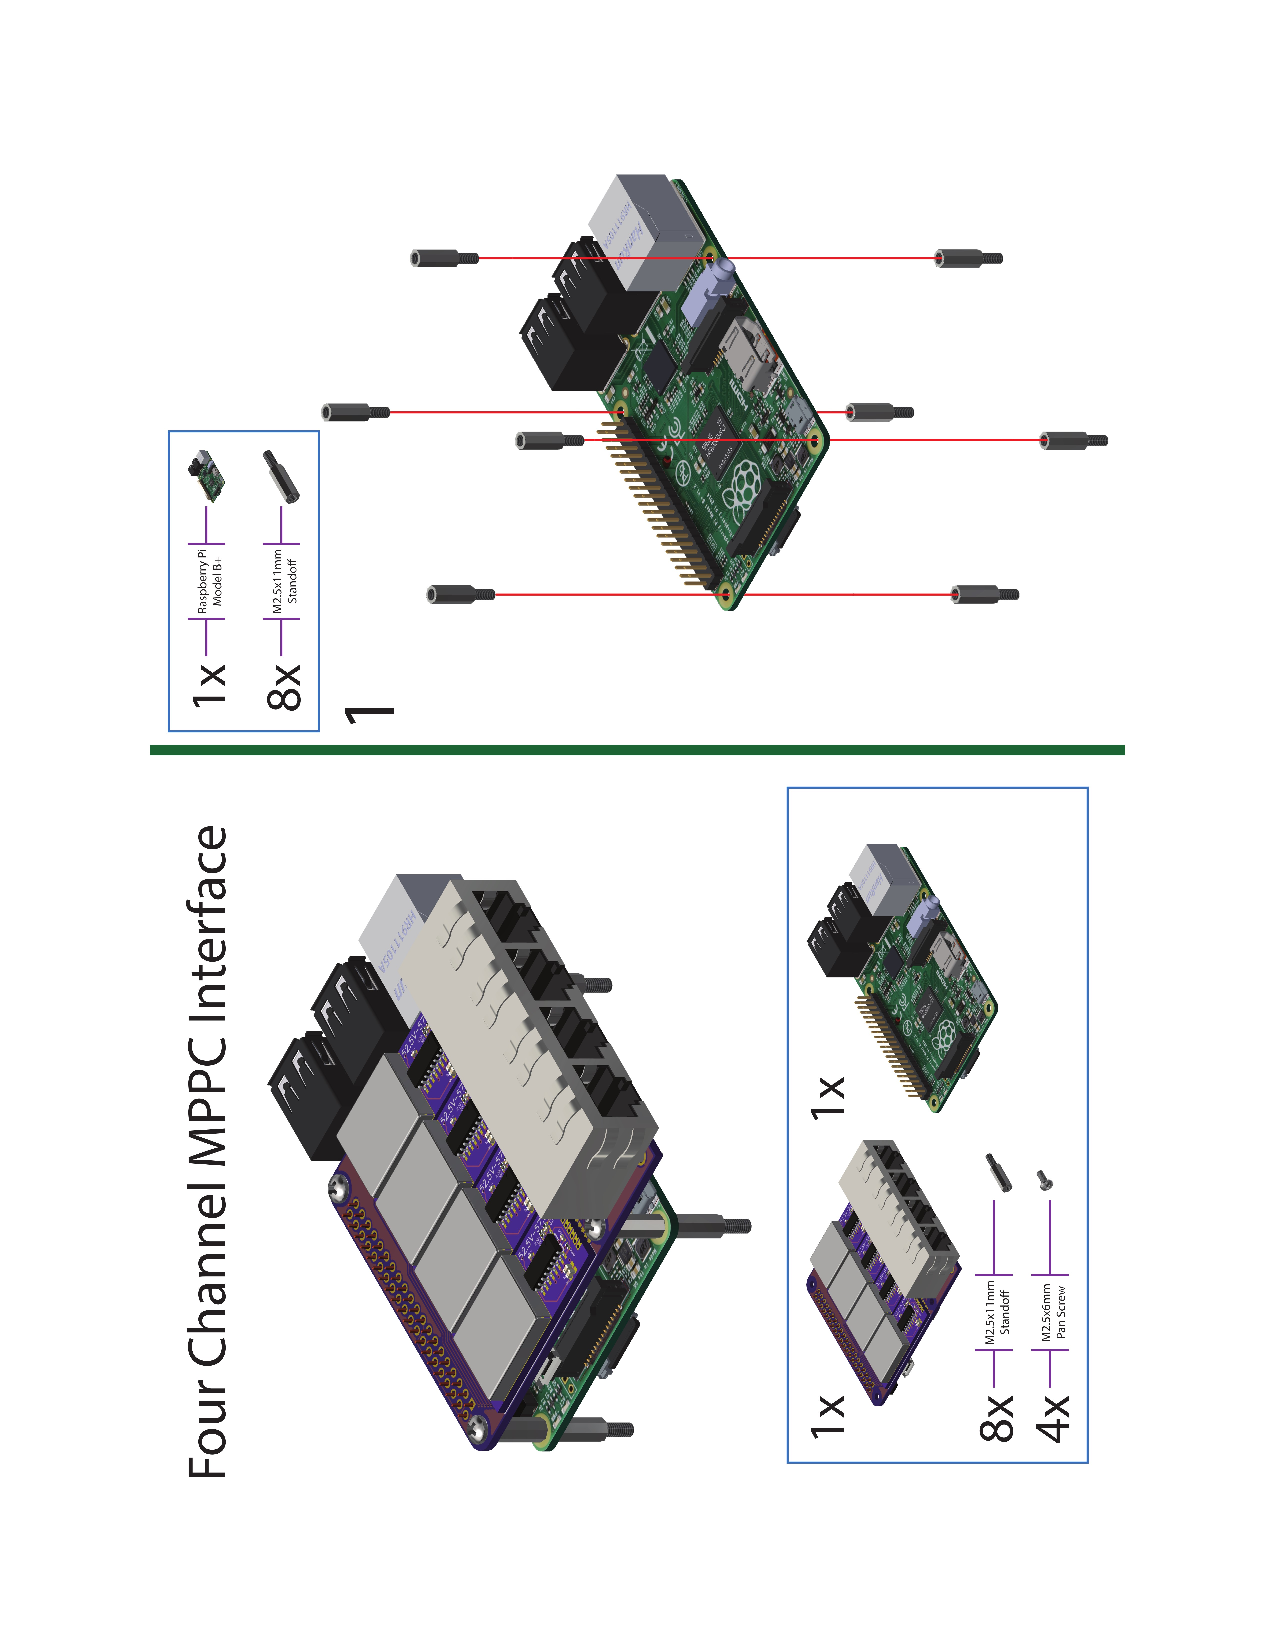
\includepdf[pages={ - }]{./tex/assembly/mppcInterfaceAssembly.pdf}
\includepdf[pages={ - }]{./tex/assembly/frameAssembly.pdf}

\chapter{Software}
\section{Structure}



\subsection{Technologies}

The application is built on many modren web technologies. This allows the applicaiton to be easily scaleable, modular, and deplyable. The following sections list the technologies and how they are used.

\subsubsection{Docker}
\href{https://www.docker.com/}{Docker} is a linux containerization platform. By created virtual containers that share the same underlying kernel, docker is able to provide an internal routing network as well as seperation and modularity of modules designed. Docker is also being used for deployment, instead of requiring the user to install multiple packages and configure them, or doing so though a makefile designed for the distro installation, we are able to target just the processor arcetecture, meaning installing docker on either a ARM or x86 processor is the only requirement. The containers are configured to install debian and then only the software required for the execution of that module, this allows debugging and testing of single modules, and removal of modules not needed for an application.

\subsubsection{Node.js}
\href{https://nodejs.org/en/}{Node.js} is a Javascript runtime built on Chrome's V8 engine. It us used for back-end processing and is the server-side languge we use. Its event driven asyncronous model allows serving multiple requests without blocking. It is also highly extensible via \href{https://www.npmjs.com/}{NPM} (Node Package Manager) which provides many modules to speed up workflow. Some of the modules we use as well as thier funcitons are shown below.

\begin{itemize}
  \item \emph{Express} - Web server for hosting dynamic content. Backbone of our REST API.
  \item \emph{Sequelize} - MySql interface that allows direct queries.
  \item \emph{RaspIO} - Input-output capabilities for the Raspberry Pi.
\end{itemize}

We also have many custom built modules such as those for communicating with the GPS module and other hardware that is specific to our design.

\subsubsection{MySQL}
\href{https://www.mysql.com/}{MySQL} is a open source relational database that is used to store and acsess data produced by the detectors. MySQL provides a convient command line interface and allows database replicaiton for .The database scheema an structure is described in its own section.

\subsubsection{Polymer}
\href{https://www.polymer-project.org/1.0/}{Polymer} is a library designed to make using web-components introducted and accepted in the latest web standards easy to use and implement. Web componets allow html imports allowing web front-ends to be built modularly. It also includes a library of web componets that follow Google's \href{https://material.io/guidelines/}{material design} guidleines preseinting a consistant style. With HTML imports, the HTML of the page is able to only fetch what it needs, and speeds up page loading. It also allows easy reuse of sections designed. Polymer also includes a data-binding system allowing communication between providied and custom built modules.

\subsubsection{NGINX}
\href{https://www.nginx.com/resources/wiki/}{NGINX} is a high preformance low recource web server. It is being used to not only serve the static content, but also to proxy-pass the requests for dynamic content and load balalcne them between the intacnes running in other containers.

\subsubsection{Firebase}
\href{https://firebase.google.com/}{Firebase} provides a full backend server management interface as well as hosting, database, and other tools. We wil be primarily using it for its user authentication. It intergrates easily into polymer, and can provide security tokens to users.

\subsubsection{Slack}
\href{https://slack.com/}{Slack} is a business focused highly intergrateable instant messaging platform designed to replace fragmented email communication. We will be using it for sending the state of the machine and getting its ip address, location and other onformation on boot.

\subsection{Architecture}
The architecture is designed in a manner to maximise the utility of all the modules and compnents created. Becasue of this the archetecture varies depending on if it is a server, a client, or takes both roles.



\subsection{Operation}

Building and running the system is fairly simple and requires a single command to bring all the docker containers up.

\begin{verbatim}
cd cosmicNetwork
sudo docker-compose up --file arm.dockercompose.yml --build
\end{verbatim}
\section{Custom Packages}
Several custom node.js packages need to be created to interface with the hardware. These are kept seperately and added via npm dependencies. They are written in javascript and designed to work with the raspberry pi. 

\begin{itemize}
  \item \href{https://github.com/muonTelescope/coincidence}{\emph{Coincidence}} - Counts number of interupts per given time period. This is used to read both the single channel and coincidence counts.
  \item \href{https://github.com/Sawaiz/mpl3115a2}{\emph{NXP MPL3115A2}} - Pressure and temprature sensor.
  \item \href{https://github.com/Sawaiz/sht3x}{\emph{Sensirion SHT3x}} - Temprature and humididty sensor.
  \item \href{https://github.com/muonTelescope/mppc-interface}{\emph{MPPC Interface}} - Sends and recives voltage, temprature, target voltage and test led data.
  \item \href{https://github.com/muonTelescope/neo6m}{\emph{uBLOX NEO6M}} - GPS module with dead reckoning.
\end{itemize}


\section{Development Tools}
The minimalist software pacakage possible are commands that can print out raw data to the terminal. The \href{https://github.com/muonTelescope/dev-tools}{dev-tools} codebase does just that. The readme for that coves how to use it.


%\input{./tex/hardware.tex}
%\input{./tex/software.tex}
%\input{./tex/operation.tex}
%\input{./tex/appendix.tex}

\pagebreak

\end{document}